%%%%%%%%%%%%%%%%%%%%%%%%%%%%%%%%%%%%%%%%%%%%%%%%%%%%%%%%%%%%%%%%%%%%%%%%%%%%
% AGUJournalTemplate.tex: this template file is for articles formatted with LaTeX
%
% This file includes commands and instructions
% given in the order necessary to produce a final output that will
% satisfy AGU requirements, including customized APA reference formatting.
%
% You may copy this file and give it your
% article name, and enter your text.
%
%
% Step 1: Set the \documentclass
%
% There are two options for article format:
%
% PLEASE USE THE DRAFT OPTION TO SUBMIT YOUR PAPERS.
% The draft option produces double spaced output.
%

%% To submit your paper:
\documentclass[draft]{agujournal2019}
\usepackage{url} %this package should fix any errors with URLs in refs.
\usepackage{lineno}
\usepackage{color}
\graphicspath{ {figures/} }
\linenumbers
%%%%%%%
% As of 2018 we recommend use of the TrackChanges package to mark revisions.
% The trackchanges package adds five new LaTeX commands:
%
%  \note[editor]{The note}
%  \annote[editor]{Text to annotate}{The note}
%  \add[editor]{Text to add}
%  \remove[editor]{Text to remove}
%  \change[editor]{Text to remove}{Text to add}
%
% complete documentation is here: http://trackchanges.sourceforge.net/
%%%%%%%

\draftfalse

%% Enter journal name below.
%% Choose from this list of Journals:
%
% JGR: Atmospheres
% JGR: Biogeosciences
% JGR: Earth Surface
% JGR: Oceans
% JGR: Planets
% JGR: Solid Earth
% JGR: Space Physics
% Global Biogeochemical Cycles
% Geophysical Research Letters
% Paleoceanography and Paleoclimatology
% Radio Science
% Reviews of Geophysics
% Tectonics
% Space Weather
% Water Resources Research
% Geochemistry, Geophysics, Geosystems
% Journal of Advances in Modeling Earth Systems (JAMES)
% Earth's Future
% Earth and Space Science
% Geohealth
%
% ie, \journalname{Water Resources Research}

\journalname{JGR: Space Physics}


\begin{document}

\title{Microburst Scale Size Distribution Derived with AeroCube-6}

%% ------------------------------------------------------------------------ %%
%
%  AUTHORS AND AFFILIATIONS
%
%% ------------------------------------------------------------------------ %%

\authors{M. Shumko\affil{1}, T.P. O'Brien\affil{2}, J. Sample\affil{1}, A. Johnson\affil{1}, D.L. Turner\affil{2}, J.B. Blake\affil{2}, B.A. Griffith\affil{1}, O. Agapitov\affil{3}, S. Claudepierre\affil{2}}


\affiliation{1}{Department of Physics, Montana State University, Bozeman, Montana, USA}
\affiliation{2}{Space Science Applications Laboratory, The Aerospace Corportation, El Segundo, California, USA}
\affiliation{3}{Space Sciences Laboratory, University of California berkeley, Berkeley, California, USA}

\correspondingauthor{M. Shumko}{msshumko@gmail.com}

%% Keypoints, final entry on title page.
%  List up to three key points (at least one is required)
%  Key Points summarize the main points and conclusions of the article
%  Each must be 100 characters or less with no special characters or punctuation and must be complete sentences

\begin{keypoints}
\item The microburst size distribution in low Earth orbit and the magnetic equator was estimated.
\item In low Earth orbit the majority of microbursts have a scale size on the order of a few tens of km.
\item At the magnetic equator the size of most microbursts correspond to the scale of \textcolor{red}{highly} correlated and \textcolor{red}{high amplitude?} whistler-mode chorus waves.
\end{keypoints}

%% ------------------------------------------------------------------------ %%
%
%  ABSTRACT
%
% A good abstract will begin with a short description of the problem
% being addressed, briefly describe the new data or analyses, then
% briefly states the main conclusion(s) and how they are supported and
% uncertainties.
%% ------------------------------------------------------------------------ %%

%% \begin{abstract} starts the second page

\begin{abstract}
Microbursts are an impulsive increase of electrons from the radiation belts into the atmosphere and has been directly observed in low Earth orbit and upper atmosphere. Microburst are believed to be generated by wave-particle scattering between whistler mode waves and radiation belt electrons. Prior work has estimated that microbursts are capable of rapidly depleting the radiation belt electrons on the order of a day, hence their role to radiation belt electron losses must be considered. Radiation belt electron losses due to microbursts is not well understood, and more work is necessary to accurately quantify their contribution. To further address this question we present a statistical study of microburst scale sizes using the pair of AeroCube-6 CubeSats. The microburst scale size distribution in low Earth orbit and the magnetic equator was derived. In low Earth orbit, \textcolor{red}{the majority of microbursts were found to have a size of less than a few tens of km with a minority of microbursts observed at a separation above 50 km. When mapped to the magnetic equator, the microburst scale size distribution corresponds to highly correlated and high amplitude ($> X$ pT) whistler mode chorus scale size derived in prior literature.}
\end{abstract}

\section{Plain Language Summary}
https://sharingscience.agu.org/creating-plain-language-summary/

\section{Introduction}
Since the discovery of the Van Allen radiation belts in the 1960s by \citeA{Allen1959} and \citeA{Vernov1960}, decades of research has made headway in understanding the dynamics particle acceleration and loss mechanisms. One of acceleration and loss mechanisms extensively studied is wave-particle scattering between whistler-mode chorus waves and electrons \cite{Abel1998_1, Meredith2002, Horne2003, Thorne2005, Millan2007, Bortnik2008}. Whistler-mode chorus waves are typically generated by a temperature anisotropy of low energy electrons up to tens of kiloelectronvolts (keV) and are typically found in the $\sim 6-12$ magnetic local times (MLT) \cite{Li2009, Li2009b}. Whistler-mode chorus waves interact with radiation belt electrons, and are widely believed to cause electron precipitation termed microbursts \cite{Millan2007}

Microbursts are a subsecond impulse of electrons that are observed by high altitude balloons and satellites in low Earth orbit (LEO) on the radiation belt magnetic footprints, $\sim 4 - 8$ L-shell (L) \cite{Anderson1964, Parks1967, Lorentzen2001a, Lorentzen2001b, O'Brien2003, Woodger2015, Crew2016, Breneman2017, Mozer2018, Greeley2019}. Microburst`s role as a radiation belt electron loss mechanism has been estimated to be significant, with total radiation belt electron depletion due to microbursts estimated to be on the order of a day \cite{Lorentzen2001b, O'Brien2004, Thorne2005, Breneman2017}. 

One of the unconstrained microburst parameters that is critical to better quantify the role of microbursts as a loss mechanism is their physical size. Historically there have been various case studies that estimated microburst size. \citeA{Parks1967} found that the size of mostly low energy microbursts to be $40 \pm 14$ km. \citeA{Blake1996} found a microburst with a size of a few tens of km using the the Solar Anomalous and Magnetospheric Particle Explorer (SAMPEX) and concluded that typically microbursts are less than a few tens of electron gyroradii in size (order of a few km in LEO). \citeA{Dietrich2010} also used SAMPEX in another case study and concluded that the observed microbursts were smaller than $4$ km. More recently, \citeA{Crew2016} used the Focused Investigation of Relativistic Electron Bursts: Intensity, Range, and Dynamics (FIREBIRD-II) CubeSats and found an example of a microburst larger than 11 km, and \citeA{Shumko2018a} used FIREBIRD-II to identify a microburst with a size greater than $ 51 \pm 1$ km. The large variance in prior results imply that there is a distribution of microburst scale sizes that this study aims to estimate.

Besides addressing the microburst role in radiation belt electron losses, the microburst size distribution is pertinent to identify the wave mode(s) responsible for scattering microbursts. The microburst size distribution in LEO can be mapped to the magnetic equator and the mapped microburst size distribution compared to various wave scales derived in prior literature to identify the dominant wave properties responsible for scattering microburst electrons. 

This study addresses these two questions by estimating the microburst size distribution in LEO and the magnetic equator. The twin AeroCube-6 (AC6) CubeSats are utilized for this study because they are ideally equipped for observing microbursts and they took data simultaneously over a span of three years while their separation varied between 2 and 800 km. This paper first describes the AC-6 mission, including their orbit and instrumentation. Then the procedure undertaken to identify microbursts observed by each spacecraft and how they are combined to make a list of the temporally coincident microbursts is described. Next, the microburst size distributions in LEO and the magnetic equator as a function of spacecraft separation is derived. Then a model is developed to understand how various microburst size distributions will be seen by a two-point measurement. Lastly, we discuss and summarize these results and infer the properties of the whistler-mode chorus waves that are believed to cause microbursts. 

\section{Instrumentation}
The AC6 mission consists of a pair of 0.5U (10x10x5 cm) CubeSats built by the Aerospace Corporation and launched on June 19th, 2014 into a 620 x 700 km, 98 degree inclination orbit. The two satellites, designated as AC6-A and AC6-B separated after launch and drifted apart. AC6 has an active attitude control system which allows them to change their differential drag to allow fine separation control. Figure 1a shows the AC6 separation for the duration of the mission.

Each AC6 unit is equipped with a three Aerospace microdosimeters (licensed to Teledyne Microelectronics, Inc). The dosimeter used for this study is dos1 and is identical on both AC6 units. Dos1 has a 30 keV electron threshold and samples at 10 Hz. The AC6 orbit is in the dawn-dusk MLT sectors and Fig. 1b shows the number of quality 10 Hz samples taken simultaneously by AC6 as a function and L and MLT. Quality samples have a 0 data quality flag. The quality flag and detailed technical information on AC6 is described in \citeA{O'brien2016}.

\begin{figure}
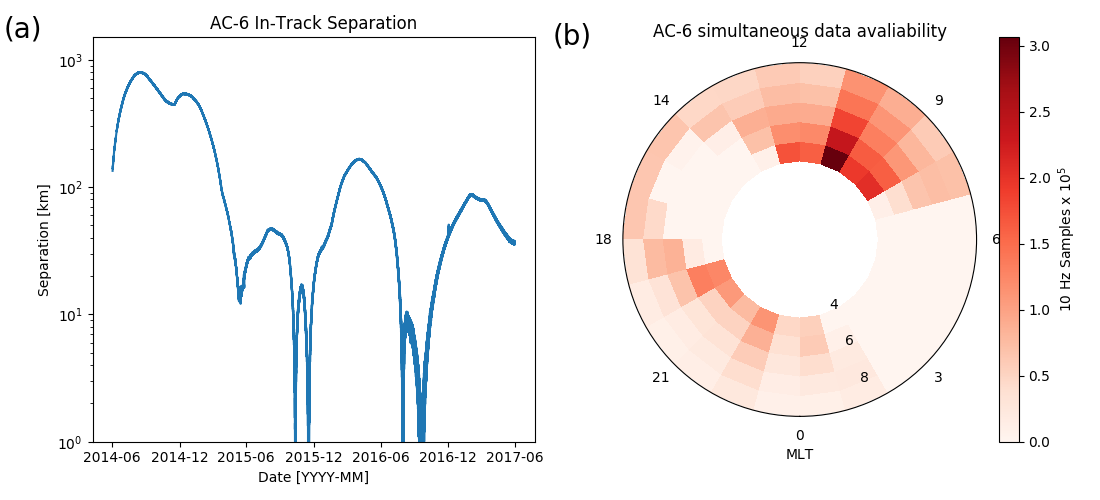
\includegraphics[width=\textwidth]{fig1.png}
\caption{AC6 mission distributions for (a) spacecraft separation and (b) number of simltaneous 10 Hz samples as a function of L and MLT.} \label{fig1}
\end{figure}

\section{Methodology}
\subsection{Microburst Detection}
The first step to find microbursts observed simultaneously by both spacecraft is to identify them from each spacecraft separately. We have detected microbursts with two different methods that yielded quantitatively similar results. The first method is the burst parameter \cite{O'Brien2003}. This algorithm has been successfully used in other microburst studies, mainly with the microbursts observed by the Solar Anomalous and Magnetospheric Particle Explorer add citations. For AC6, we found that a burst parameter threshold of 5 has good tradeoff between false positive and false negative microburst detections. \textcolor{red}{Talk about the wavelet based detector as well?}

The transmitters on AC6 can cause unphysical count impulses in the dosimeters that resembles periodic trains of microbursts. These false detections were removed to remove their bias. One source of transmitter noise was observed at times when AC6 was in contact with the ground stations above mainland US for data downloads and commanding thus the mostly low L detections made above the US were discarded. 

Another source of noise is crosslink transmissions between the AC6 units. These transmissions occurred when either spacecraft transitioned from the survey mode to 10 Hz mode. This noise is sometimes not caught by the data quality flag, so the following empirically-derived criteria was developed to remove those detections. The dosimeter with a 250 keV nominal electron threshold, dos2 was used because it had a similar response to noise while rarely responded to microbursts. Since the transmitter noise is very periodic, cross-correlation (CC) and autocorrelation (AC) methods were applied to the dos1 and dos2 time series. Detections were removed if the following two criteria were met: either dos1 or dos2 time series had a AC peak at a 0.2 or 0.4 s lag, and the dos1-dos2 CC was greater than 0.9. The AC lag criteria alone sometimes falsely removed legitimate trains of microbursts, so the second criteria insured that the detection was removed if there was a very high correlation across an order of magnitude in energy.

The lists of microbursts observed by either AC6 unit were merged into a temporally coincident list with the following procedure. \textcolor{red}{Show the microburst detection cartoon I`ve showed in conferences?} The general idea is that a microburst detection on one spacecraft will CC well will the time series from the other spacecraft if it observed a similar microburst, and poorly if there was no microburst observed by the other spacecraft. Each microburst detection made by either spacecraft was CC with the time series from the other spacecraft. Windows of 1 and 1.2 s were used to CC the time series. Different window sizes were used to account for numerical uncertainty due to Poisson noise. Microbursts detections with a CC above 0.8 were considered temporally coincident. This CC threshold was chosen as it is low enough to identify temporally coincident microbursts superposed with noise, and high enough to reject most non-coincident events. Figure \ref{fig2}, panels (a), (c), and (e) show examples of microbursts observed by both AC6 units when they were separated by 6, 17, and 69 km, respectively. 

The last CC criteria required that the temporal CC must be greater than the spatial CC + 0.3. The spatial CC was calculated by shifting the AC6-B time series by the in-track lag to CC in latitude. This criteria was applied to remove curtains, spatially stationary and narrow in latitude structures obsered by AC6 \cite{Blake2016} and sometimes appear as microbursts. Figure \ref{fig2}, panels (b), (d), and (f) show the AC6 spatially aligned time series to confirm that the three cases shown were indeed microbursts. The coincident microburst list was then spot checked by two authors to any remove poorly correlated events. Considering the CC criteria and data availability, 662 confirmed simultaneous microburst detections are used to calculate the microburst size distribution in the following section.

\begin{figure}
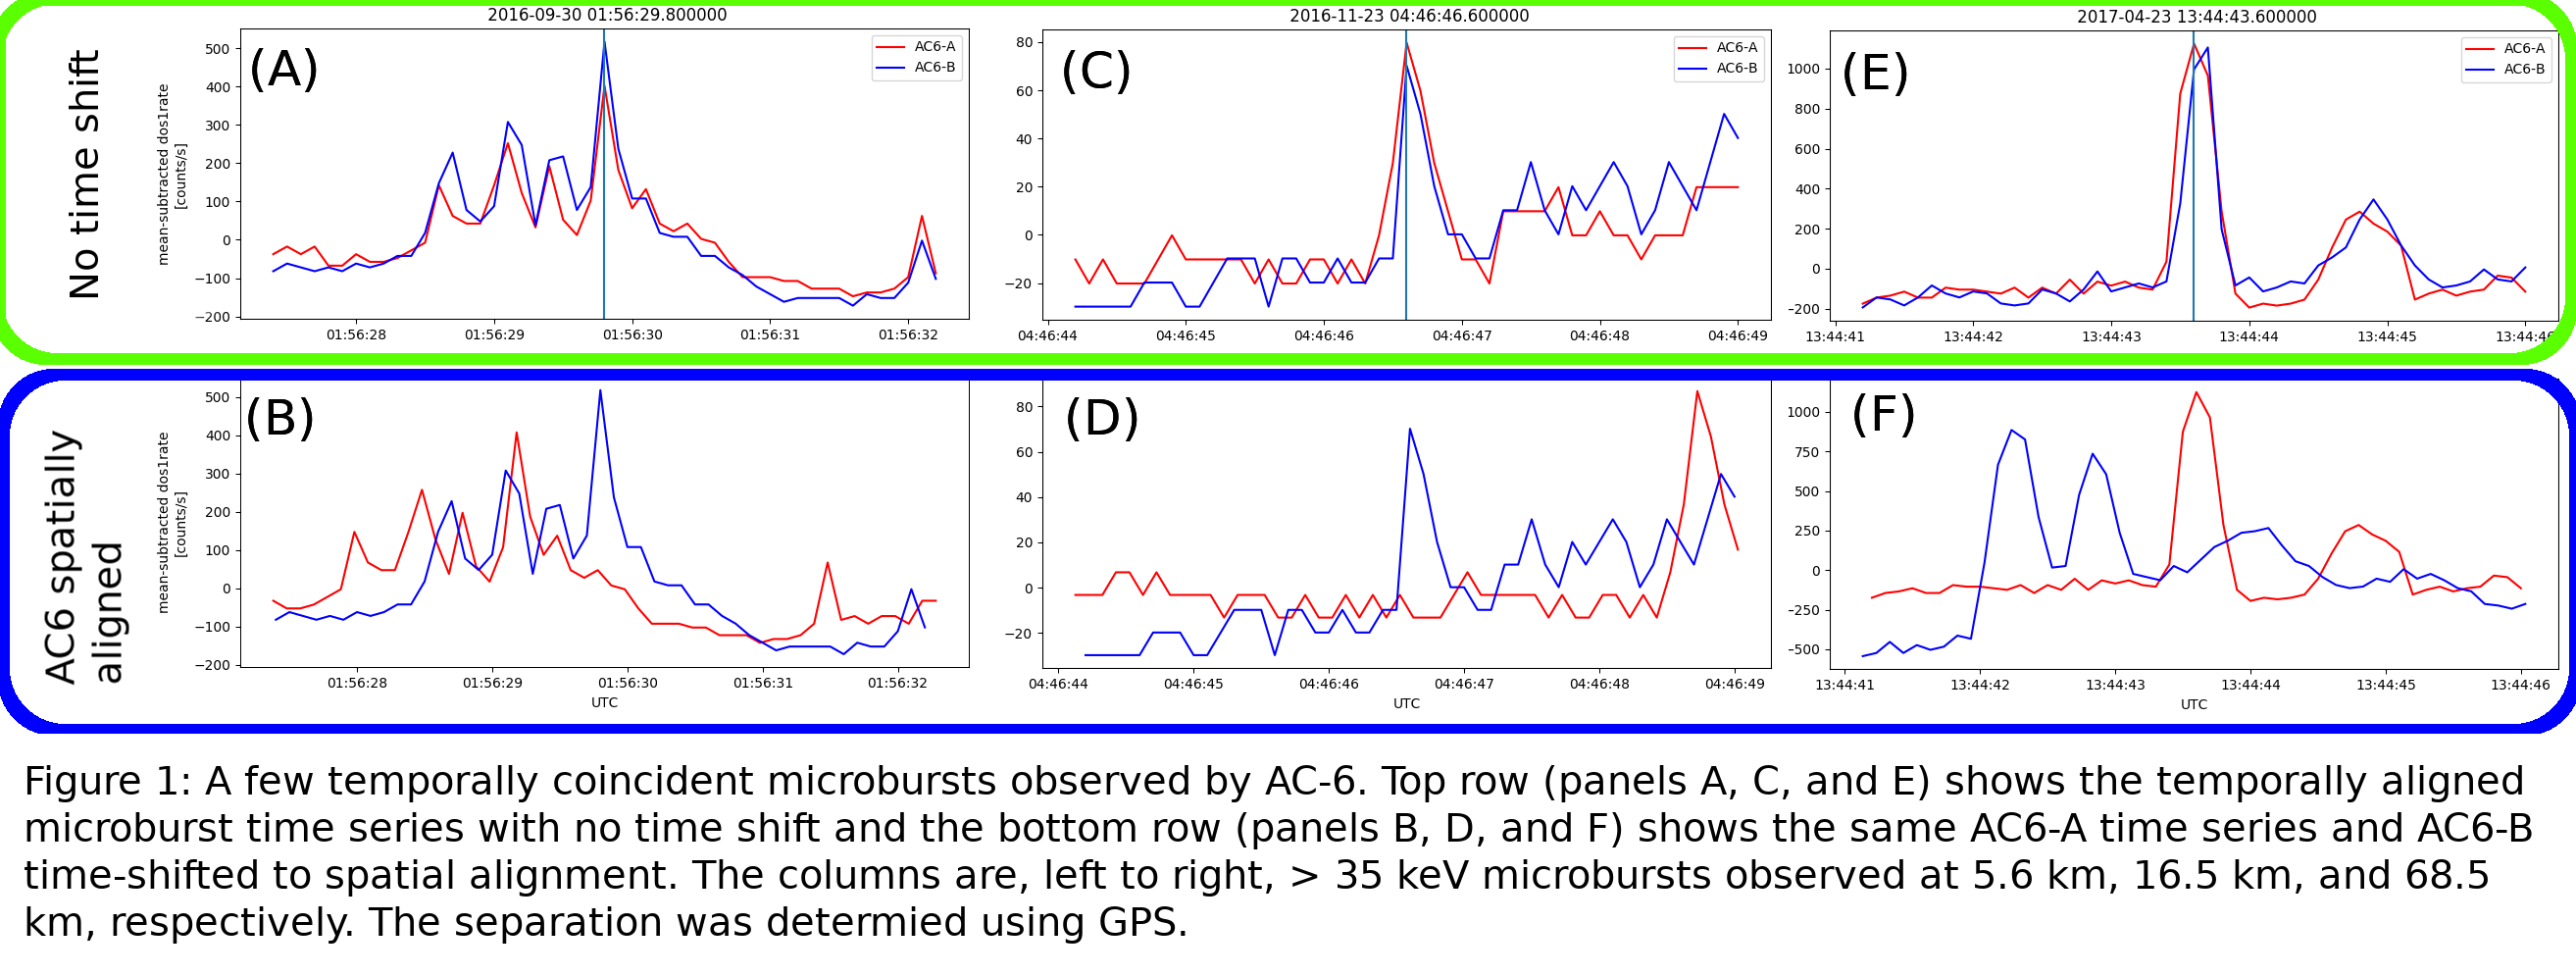
\includegraphics[width=\textwidth]{fig2.png}
\caption{Examples of microbursts observed simultaneously by AC6. Panels (a), (c) and (e) shows the temporally-aligned time series at spacecraft separations of 5.6 km, 16.5 km, and 68.5 km, respectively. Panels (b), (d), and (f) show the spatially aligned time series corresponding to the time series in the same column. The clear temporal correlation and lack of spatial correlation demonstrates that these events are microbursts.} 
\label{fig2}
\end{figure}
	

\subsection{Microburst Size Distribution in LEO and Magnetic Equator}\label{microburst_distribution}
The list of temporally coincident microbursts, which from now on will just be called microbursts, is now compiled to show the fraction of microbursts observed above a separation $s$. When AC6 observes a microburst at $s$, the microburst`s size must be greater than $s$. This fact, along with the arguments presented in Section 4 in \citeA{Joy2002}, is used to investigate the dependence of the number of microbursts observed above $s$, as a function of $s$ which is the microburst complementary cumulative distribution $F(s)$. 

\textcolor{red}{Include the following Bayes theorem proof? It does not seem necessary (or I did not motivate it)} If P(A) is the probability that a microburst is larger than $s$ and P(B) is the probability that AC6 is separated by $s$, then the fraction of microbursts observed at $s$ is the conditional probability $P(A \ \vert \ B)$. Using Bayes’ theorem, 
\begin{equation}
P(A \ \vert \ B) = \frac{P(A \ \& \ B)}{P(B)}
\end{equation} where $P(A \ \& \ B)$ is the joint probability. Since the AC6 separation is independent of microburst size, $P(A \ \& \ B) = P(A)P(B)$. Hence

\begin{equation}
P(A \ \vert \ B) = \frac{P(A)P(B)}{P(B)} = P(A)
\end{equation} so AC6 is observing the probability that the microburst is larger than $s$.

The cumulative number of microbursts observed above $s$ is the ratio of $N(s)$, the number of microbursts observed above $s$ to $N(0)$, the total number of microbursts observed 
\begin{equation}
F(s) = \frac{N(s)}{N(0)}
\end{equation} 

\begin{equation}
N(s) = \sum_{i = s}^\infty n_{i} \frac{S_{max}}{S_{i}}
\end{equation} where $n_{i}$ is the number of microbursts observed by AC6 in ith bin. The normalization term $S_{max}/S_{i}$ is a ratio of the number of samples observed in the most sampled bin to the number of samples in ith bin. This normalization factor corrects for AC6's non-uniform sampling in separation and the number of samples is shown in Fig. \ref{fig3}c. With this normalization, $F(s)$ can be interpreted as the fraction of microbursts observed above $s$ assuming AC6 sampled evenly in separation. Microburst $F(s)$ in LEO is shown by the black curve in Fig. \ref{fig3}a for $4 < \mathrm{L}< 8$ and split into one L-wide bins with the colored curves. The separation bin width used in Fig. \ref{fig3} is 5 km. To check for bias in $F(s)$ due to the separation bins, $F(s)$ was resampled with other bin widths and offsets. Bin widths as large as the size of the features in $F(s)$ ($20-30$ km) and bin offsets up to $50\%$ of the bin width did not qualitatively effect the curves in Fig. \ref{fig3}a.

The overall trend in Fig. \ref{fig3}a consists of a sudden cumulative probability drop off, followed by a shoulder up to $s \approx 70$ km where the cumulative distribution drops to nearly zero. The shaded region around the black curve shows the standard error due to counting statistics. The uncertainty due to false coincidence events i.e. two unrelated microbursts randomly lining up in time was also considered. The microburst duty cycle in a one minute window ($\approx 1 \ L$) around each microburst was calculated. The false coincidence probability is the square of the duty cycle and was found to be less than 5\% for the majority of microbursts. The false coincidence probability for each microburst was then used to randomly remove microbursts and $F(s)$ was recalculated in $1000$ trials. The uncertainty in $F(s)$ with microbursts randomly removed was much smaller than the uncertainty due to counting statistics alone. Lastly, Fig. \ref{fig3}b shows the microburst probability density (PD), calculated by differentiating $F(s)$, and shows a peak at $s < 20 $ km as well as a peak between 70-80 km separation. 

To compare the microburst size to the size of their progenitor waves, the spacecraft locations during observed microbursts were mapped to the magnetic equator using the Olson-Pfitzer magnetic field model \cite{Olson1982} which is implemented with a Python wrapper for IRBEM-Lib \cite{irbem}. As previously stated, a microburst observed in LEO has a size larger than the spacecraft separation, hence that microburst would also have a size larger than the spacecraft separation after it was mapped to the magnetic equator. Thus the procedure to estimate $F(s)$ is identical to the LEO size distribution but with a different normalization. The normalization factors were calculated by mapping every quality AC6 sample taken simultaneously to the magnetic equator and binning them by equatorial separation into 100 km bins. Figure \ref{fig4} shows the equatorial microburst size distribution in the same format as Fig. \ref{fig3}. Similar to the microburst PD in LEO, most of the equatorial microburst PD was observed when the AC6 equatorial separation was less than 300 km. 

The results in Figs. \ref{fig3} and \ref{fig4} show the fraction of microbursts observed above a spacecraft separation and do not fully represent the microbursts size distribution due to the compounding effects from the range of microburst sizes and random locations of microbursts with respect to AC6 i.e. even if the microburst size is much larger than $s$, a fraction of those microbursts will graze only one AC6 unit and not be observed by the other. Thus modeling is necessary to capture the compounding influence of these statistical effects on AC6, a two-point measurement.

\begin{figure}
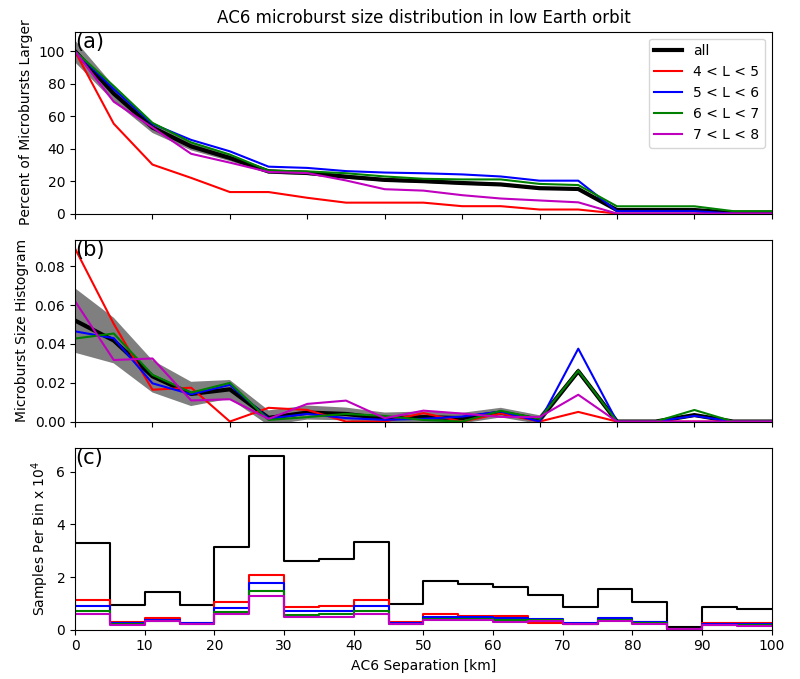
\includegraphics[width=\textwidth]{fig3.png}
\caption{Fraction of microbursts greater than the spacecraft separation as a function of separation in LEO. Panel (a) shows the fraction of microbursts observed above that separation. Panel (b) shows the microburst probability density as a function of separation. Lastly, panel (c) shows the number of simultaneous samples AC6 observed as a function of separation. The colored lines show the distributions binned by L, and the thick black curve shows the fraction of microbursts observed above a separation in the entire radiation belt ($4 < L < 8$). The gray shading around the black curve shows the uncertainty due to counting statistics.}
\label{fig3}
\end{figure}

\begin{figure}
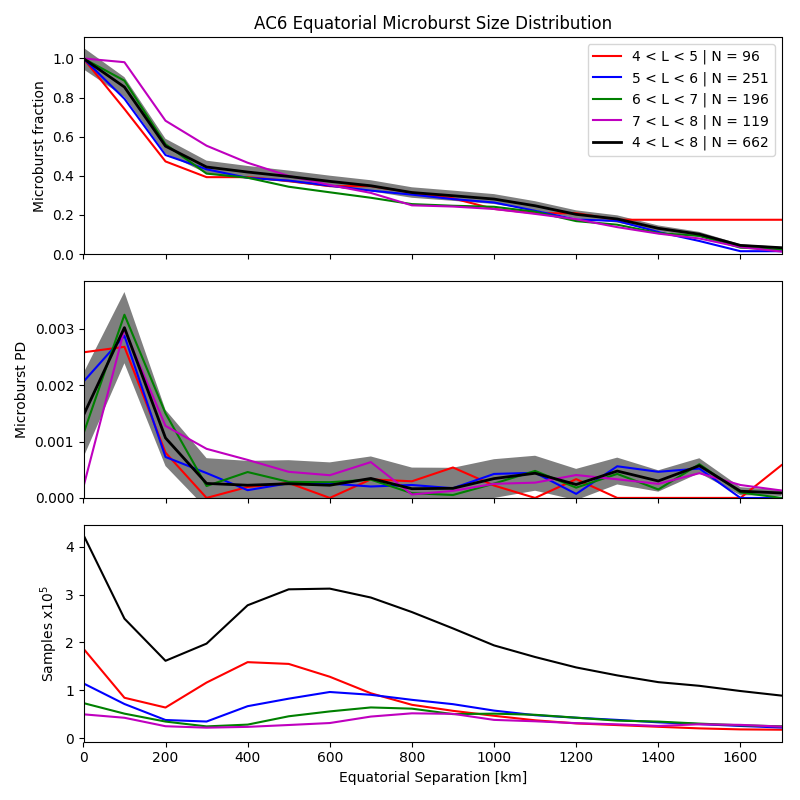
\includegraphics[width=\textwidth]{fig4.png}
\caption{Microburst scale size distribution in the same format as Fig. \ref{fig3} and mapped to the magnetic equator.} 
\label{fig4}
\end{figure}

\section{Modeling the Distribution of Microburst Sizes}
\subsection{Monte Carlo and Analytic Models to Estimate $F(s)$}
\textcolor{blue}{
TO-DO
\begin{itemize}
\item Show a LEO CDF model assuming a fixed-sized microburst population.
\item Decide if I should show a two-fixed-sized microburst population or a microburst CDF.
\item Show the residuals in the plots.
\item Think about a model comparison.
\end{itemize}
}

To account for the effects due to microbursts randomly occurring in the vicinity of AC6 with an unknown distribution of microburst sizes, Monte Carlo (MC) and analytic models were developed. These models assume a hypothesized distribution of microburst sizes expressed with a probability density function $P(r)$, and a microburst geometry to estimate $F(s)$. Microbursts are assumed to be circular with a radius $r$. A few distribution of microburst size hypotheses are considered: a one-size microburst population, a two-size microburst population, and \textcolor{red}{X} continuous $P(r)$.

The MC model is the most intuitive to understand and it consists of randomly scattering $10^5$ microburst centers in a 400 x 400 km grid around AC6 of various $r$ that are distributed according to $P(r)$. Spacecraft A is placed at the origin, and spacecraft B is placed along the positive y-axis at predetermined distances from the origin corresponding to he AC6 separation bins used in Section \ref{microburst_distribution} Then the cumulative number of simultaneously observed microbursts at spacecraft A and each spacecraft B location was counted. The modeled fraction of microbursts observed above $s$ is then
\begin{equation}
F(s) = \frac{\displaystyle\sum_{i > s}^\infty n_{i} }{ \displaystyle\sum_{i > 0}^\infty n_{i} }.
\end{equation} where as before the number of microbursts observed by both spacecraft in ith bin is $n_{i}$. 

The analytic model, while identical to the MC model, highlights the geometrical concepts connecting the microburst size distribution and $F(s)$. Assuming that microbursts are circular with radius $r$ and AC6 are separated by $s$, there is an area where a microburst will be observed by both spacecraft. Figure \ref{fig5}a shows this geometry with the two spacecraft indicated with the black dots. All microbursts who's center lies inside the circular area of radius $r$ that surrounds the top spacecraft will be observed by the top spacecraft. Likewise the same argument applies to the bottom spacecraft. The intersection of these two areas defines another area, $A(r, s)$ where a microburst will be observed by both spacecraft and is given by the circle-circle intersection area equation, 
\begin{equation}
A(r, d) = 2r^2 \cos^{-1}{\Big( \frac{d}{2r} \Big)} - \frac{d}{2} \sqrt{4r^2 - d^2}.
\end{equation} \textcolor{red}{Cite anything? Wolfram: http://mathworld.wolfram.com/Circle-CircleIntersection.html} Example geometries with an overlapping area are shown in Fig. \ref{fig5}b, c.

The circle intersection area can be thought of as a probability that a microburst will be observed by both spacecraft, given that it was observed by one. The hypothesized $P(r)$ can be thought of as the relative occurrence of microbursts at various $r$ and is effectively a weighting factor on $A(r, s)$ which is integrated out (marginalized) since AC6 is observing the overall effect of microbursts at all $r$. Lastly, a cumulative integral over a dummy variable $s'$ is applied to the normalized areas to calculate $F(s)$. With these considerations the analytic $F(s)$ is given by

\begin{equation} \label{analytic_integral}
F(s) = \frac{\displaystyle\int\displaylimits_{s}^{\infty} \displaystyle\int\displaylimits_0^{\infty} A(r, s') P(r) dr ds'}{\displaystyle\int\displaylimits_{0}^{\infty} \displaystyle\int\displaylimits_0^{\infty} A(r, s') P(r) dr ds'} .
\end{equation} where as in the MC model the denominator is the normalization factor. To illustrate the effects of random microburst locations around AC6, example analytic and MC model $F(s)$ assuming a fixed-size 40 km diameter microburst population is shown in Fig. \ref{fig5}d with the dashed blue and red curves, respectively.

\begin{figure}
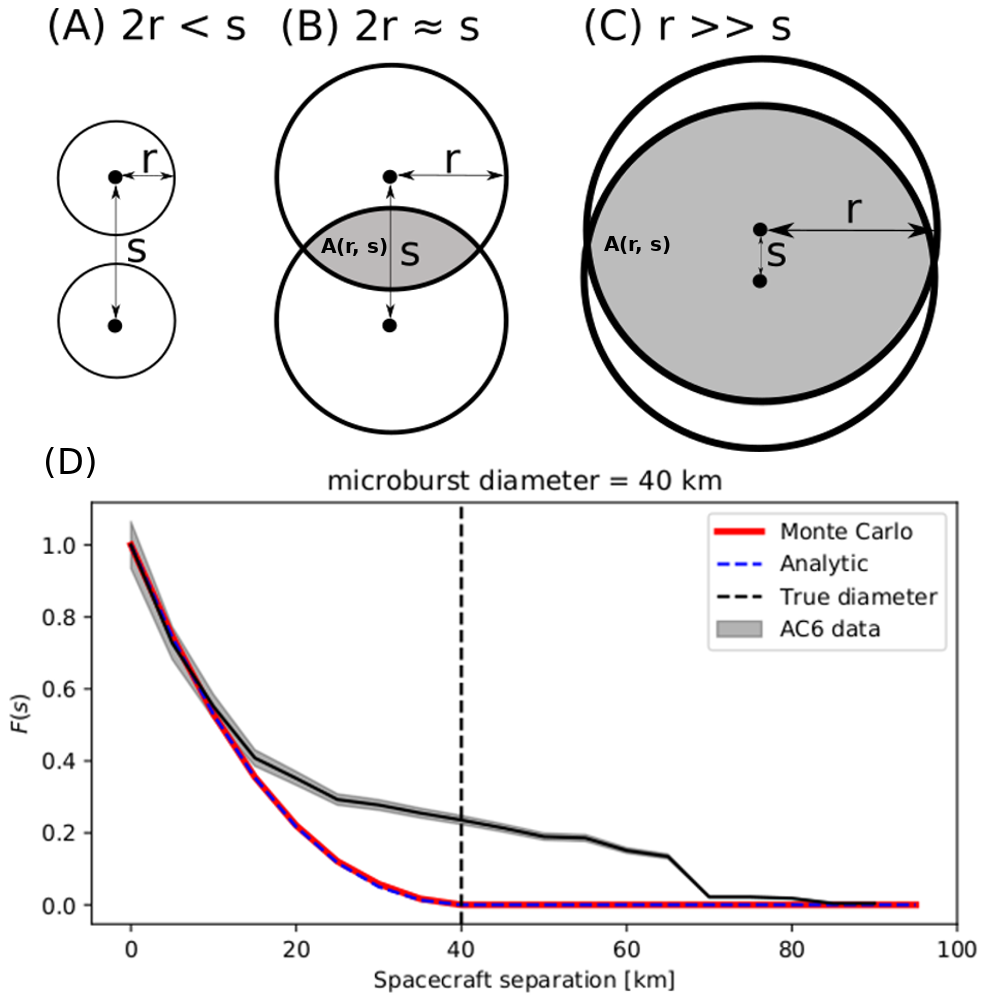
\includegraphics[width=\textwidth]{fig5.png}
\caption{Panels A-C show the geometry of the analytic model. The two spacecraft are shown as black dots. The enclosing black circle around each spacecraft bounds the area where a microburst will be observed by one or both AC6 units if the microburst's center lies inside the circle. Panel (A) shows the case where microburst diameter is smaller than the AC6 separation and all microbursts will be observed by either unit A or B and never simultaneously. Panel (B) shows the intermediate case where the microburst diameter is comparable to the AC6 separation and some fraction of microbursts will be observed simultaneously. The fraction of the microbursts simultaneously observed is proportional to the circle intersection area shown with grey shading. Panel (C) shows the case where the spacecraft separation is much smaller than the microburst size and nearly all microbursts will be observed by both spacecraft. Lastly panel (D) shows $F(s)$ from the AC6 data with a solid black line, and a MC and analytic $F(s)$ for a single-sized microburst distribution with a 40 km diameter.} 
\label{fig5}
\end{figure}

\subsection{Estimating optimal parameters for microburst size models}
At this stage a few hypothesized microburst size distributions are tested and optimal model parameters estimated. For each hypothesized microburst size distribution, Bayesian inference is used to estimate the optimal model parameters with a Metropolis Markov Chain Monte Carlo (MCMC) sampler \cite{Metropolis1953}. Bayes theorem is central to Bayesian inference and for data $d$ and model parameters $x$ can be written as

\begin{equation}
P(x | d) = \frac{P(d | x) P(x)}{P(d)}
\end{equation} where $p(x | d)$ is the posterior probability of the model parameters, given the data, $P(d | x)$ is the likelihood which returns a probability of the data given the model parameters, $p(x)$ is the prior, our knowledge about the model

The MCMC sampler sam

The MCMC sampler samples the pa




The Metropolis sampler samples the model parameter space under the following assumptions. First assumption is prior knowledge of model parameters which is called a prior and mathematically expressed with a probability density function (PDF). For the MC microburst size model uniformly and normally distributed priors are assumed. The second assumption is the likelihood function that is the probability of observed data given the model parameters. With these two assumptions the MCMC sampler iterates N times, each time picking a random set prior parameters for that particular microburst PDF. For each set of prior parameters, their prior probability is weighted by the likelihood to calculate the probability that the current set of prior parameters is explained by the data. With the Metropolis sampler, the random prior parameters are sampled in a way that is weighted by the prior and likelihood and mostly explores the regions of parameter space that is more probable.

After N trails the tested parameters as a function of trial is called a trace and the histogram of the trace is the posterior probability density of that model parameter. 

A more detailed description of the Metropolis MCMC (and its generalization to trans-dimensional inverse problems) is found in \citeA{Sambridge2006}.

\section{Discussion}
\textcolor{blue}{
TO-DO
\begin{itemize}
\item Discuss the significance of the peaks in the LEO CDF \& PDF.
\item Discuss the secondary peak.
\item Talk about how these sizes fit in with prior work and how they can be used to estimate microburst loss rates.
\item Maybe add a plot with Oleksiy's data?
\item Use the wave data to interpret the equatorial scale size distribution. Is the < 200 km peak due to high amplitude waves, or is it just that waves are most common at those scales?
\end{itemize}
}

\section{Conclusions}

%%

%  Numbered lines in equations:
%  To add line numbers to lines in equations,
%  \begin{linenomath*}
%  \begin{equation}
%  \end{equation}
%  \end{linenomath*}



%% Enter Figures and Tables near as possible to where they are first mentioned:
%
% DO NOT USE \psfrag or \subfigure commands.
%
% Figure captions go below the figure.
% Table titles go above tables;  other caption information
%  should be placed in last line of the table, using
% \multicolumn2l{$^a$ This is a table note.}
%
%----------------
% EXAMPLE FIGURE
%
%
% Giving latex a width will help it to scale the figure properly. A simple trick is to use \textwidth. Try this if large figures run off the side of the page.
% \begin{figure}
% \noindent\includegraphics[width=\textwidth]{anothersample.png}
%\caption{caption}
%\label{pngfiguresample}
%\end{figure}
%
%
%
% If you get an error about an unknown bounding box, try specifying the width and height of the figure with the natwidth and natheight options.
% \begin{figure}
% \noindent\includegraphics[natwidth=800px,natheight=600px]{samplefigure.pdf}
%\caption{caption}
%\label{pdffiguresample}
%\end{figure}
%
%
% PDFLatex does not seem to be able to process EPS figures. You may want to try the epstopdf package.
%
%
%
% ---------------
% EXAMPLE TABLE
%
% \begin{table}
% \caption{Time of the Transition Between Phase 1 and Phase 2$^{a}$}
% \centering
% \begin{tabular}{l c}
% \hline
%  Run  & Time (min)  \\
% \hline
%   $l1$  & 260   \\
%   $l2$  & 300   \\
%   $l3$  & 340   \\
%   $h1$  & 270   \\
%   $h2$  & 250   \\
%   $h3$  & 380   \\
%   $r1$  & 370   \\
%   $r2$  & 390   \\
% \hline
% \multicolumn{2}{l}{$^{a}$Footnote text here.}
% \end{tabular}
% \end{table}

%% SIDEWAYS FIGURE and TABLE
% AGU prefers the use of {sidewaystable} over {landscapetable} as it causes fewer problems.
%
% \begin{sidewaysfigure}
% \includegraphics[width=20pc]{figsamp}
% \caption{caption here}
% \label{newfig}
% \end{sidewaysfigure}
%
%  \begin{sidewaystable}
%  \caption{Caption here}
% \label{tab:signif_gap_clos}
%  \begin{tabular}{ccc}
% one&two&three\\
% four&five&six
%  \end{tabular}
%  \end{sidewaystable}

%% If using numbered lines, please surround equations with \begin{linenomath*}...\end{linenomath*}
%\begin{linenomath*}
%\begin{equation}
%y|{f} \sim g(m, \sigma),
%\end{equation}
%\end{linenomath*}

%%% End of body of article

%%%%%%%%%%%%%%%%%%%%%%%%%%%%%%%%
%% Optional Appendix goes here
%
% The \appendix command resets counters and redefines section heads
%
% After typing \appendix
%
%\section{Here Is Appendix Title}
% will show
% A: Here Is Appendix Title
%
%\appendix
%\section{Here is a sample appendix}

%%%%%%%%%%%%%%%%%%%%%%%%%%%%%%%%%%%%%%%%%%%%%%%%%%%%%%%%%%%%%%%%
%
% Optional Glossary, Notation or Acronym section goes here:
%
%%%%%%%%%%%%%%
% Glossary is only allowed in Reviews of Geophysics
%  \begin{glossary}
%  \term{Term}
%   Term Definition here
%  \term{Term}
%   Term Definition here
%  \term{Term}
%   Term Definition here
%  \end{glossary}

%
%%%%%%%%%%%%%%
% Acronyms
%   \begin{acronyms}
%   \acro{Acronym}
%   Definition here
%   \acro{EMOS}
%   Ensemble model output statistics
%   \acro{ECMWF}
%   Centre for Medium-Range Weather Forecasts
%   \end{acronyms}

%
%%%%%%%%%%%%%%
% Notation
%   \begin{notation}
%   \notation{$a+b$} Notation Definition here
%   \notation{$e=mc^2$}
%   Equation in German-born physicist Albert Einstein's theory of special
%  relativity that showed that the increased relativistic mass ($m$) of a
%  body comes from the energy of motion of the body—that is, its kinetic
%  energy ($E$)—divided by the speed of light squared ($c^2$).
%   \end{notation}




%%%%%%%%%%%%%%%%%%%%%%%%%%%%%%%%%%%%%%%%%%%%%%%%%%%%%%%%%%%%%%%%
%
%  ACKNOWLEDGMENTS
%
% The acknowledgments must list:
%
% >>>>	A statement that indicates to the reader where the data
% 	supporting the conclusions can be obtained (for example, in the
% 	references, tables, supporting information, and other databases).
%
% 	All funding sources related to this work from all authors
%
% 	Any real or perceived financial conflicts of interests for any
%	author
%
% 	Other affiliations for any author that may be perceived as
% 	having a conflict of interest with respect to the results of this
% 	paper.
%
%
% It is also the appropriate place to thank colleagues and other contributors.
% AGU does not normally allow dedications.


\acknowledgments
Enter acknowledgments, including your data availability statement, here.


%% ------------------------------------------------------------------------ %%
%% References and Citations

%%%%%%%%%%%%%%%%%%%%%%%%%%%%%%%%%%%%%%%%%%%%%%%
%
% \bibliography{<name of your .bib file>} don't specify the file extension
%
% don't specify bibliographystyle
%%%%%%%%%%%%%%%%%%%%%%%%%%%%%%%%%%%%%%%%%%%%%%%

\bibliography{/home/mike/Dropbox/0_firebird_research/A_presentations/refs}

%Reference citation instructions and examples:
%
% Please use ONLY \cite and \citeA for reference citations.
% \cite for parenthetical references
% ...as shown in recent studies (Simpson et al., 2019)
% \citeA for in-text citations
% ...Simpson et al. (2019) have shown...
%
%
%...as shown by \citeA{jskilby}.
%...as shown by \citeA{lewin76}, \citeA{carson86}, \citeA{bartoldy02}, and \citeA{rinaldi03}.
%...has been shown \cite{jskilbye}.
%...has been shown \cite{lewin76,carson86,bartoldy02,rinaldi03}.
%...has been shown \cite [e.g.,][]{lewin76,carson86,bartoldy02,rinaldi03}.
%
% DO NOT use other cite commands (e.g., \citet, \citep, \citeyear, \nocite, \citealp, etc.).
%



\end{document}



More Information and Advice:

%% ------------------------------------------------------------------------ %%
%
%  SECTION HEADS
%
%% ------------------------------------------------------------------------ %%

% Capitalize the first letter of each word (except for
% prepositions, conjunctions, and articles that are
% three or fewer letters).

% AGU follows standard outline style; therefore, there cannot be a section 1 without
% a section 2, or a section 2.3.1 without a section 2.3.2.
% Please make sure your section numbers are balanced.
% ---------------
% Level 1 head
%
% Use the \section{} command to identify level 1 heads;
% type the appropriate head wording between the curly
% brackets, as shown below.
%
%An example:
%\section{Level 1 Head: Introduction}
%
% ---------------
% Level 2 head
%
% Use the \subsection{} command to identify level 2 heads.
%An example:
%\subsection{Level 2 Head}
%
% ---------------
% Level 3 head
%
% Use the \subsubsection{} command to identify level 3 heads
%An example:
%\subsubsection{Level 3 Head}
%
%---------------
% Level 4 head
%
% Use the \subsubsubsection{} command to identify level 3 heads
% An example:
%\subsubsubsection{Level 4 Head} An example.
%
%% ------------------------------------------------------------------------ %%
%
%  IN-TEXT LISTS
%
%% ------------------------------------------------------------------------ %%
%
% Do not use bulleted lists; enumerated lists are okay.
% \begin{enumerate}
% \item
% \item
% \item
% \end{enumerate}
%
%% ------------------------------------------------------------------------ %%
%
%  EQUATIONS
%
%% ------------------------------------------------------------------------ %%

% Single-line equations are centered.
% Equation arrays will appear left-aligned.

Math coded inside display math mode \[ ...\]
 will not be numbered, e.g.,:
 \[ x^2=y^2 + z^2\]

 Math coded inside \begin{equation} and \end{equation} will
 be automatically numbered, e.g.,:
 \begin{equation}
 x^2=y^2 + z^2
 \end{equation}


% To create multiline equations, use the
% \begin{eqnarray} and \end{eqnarray} environment
% as demonstrated below.
\begin{eqnarray}
  x_{1} & = & (x - x_{0}) \cos \Theta \nonumber \\
        && + (y - y_{0}) \sin \Theta  \nonumber \\
  y_{1} & = & -(x - x_{0}) \sin \Theta \nonumber \\
        && + (y - y_{0}) \cos \Theta.
\end{eqnarray}

%If you don't want an equation number, use the star form:
%\begin{eqnarray*}...\end{eqnarray*}

% Break each line at a sign of operation
% (+, -, etc.) if possible, with the sign of operation
% on the new line.

% Indent second and subsequent lines to align with
% the first character following the equal sign on the
% first line.

% Use an \hspace{} command to insert horizontal space
% into your equation if necessary. Place an appropriate
% unit of measure between the curly braces, e.g.
% \hspace{1in}; you may have to experiment to achieve
% the correct amount of space.


%% ------------------------------------------------------------------------ %%
%
%  EQUATION NUMBERING: COUNTER
%
%% ------------------------------------------------------------------------ %%

% You may change equation numbering by resetting
% the equation counter or by explicitly numbering
% an equation.

% To explicitly number an equation, type \eqnum{}
% (with the desired number between the brackets)
% after the \begin{equation} or \begin{eqnarray}
% command.  The \eqnum{} command will affect only
% the equation it appears with; LaTeX will number
% any equations appearing later in the manuscript
% according to the equation counter.
%

% If you have a multiline equation that needs only
% one equation number, use a \nonumber command in
% front of the double backslashes (\\) as shown in
% the multiline equation above.

% If you are using line numbers, remember to surround
% equations with \begin{linenomath*}...\end{linenomath*}

%  To add line numbers to lines in equations:
%  \begin{linenomath*}
%  \begin{equation}
%  \end{equation}
%  \end{linenomath*}



